% !TEX root = ../Diplombericht.tex
\subsection{Technischer Überblick}
\begin{figure}[H]
\centering
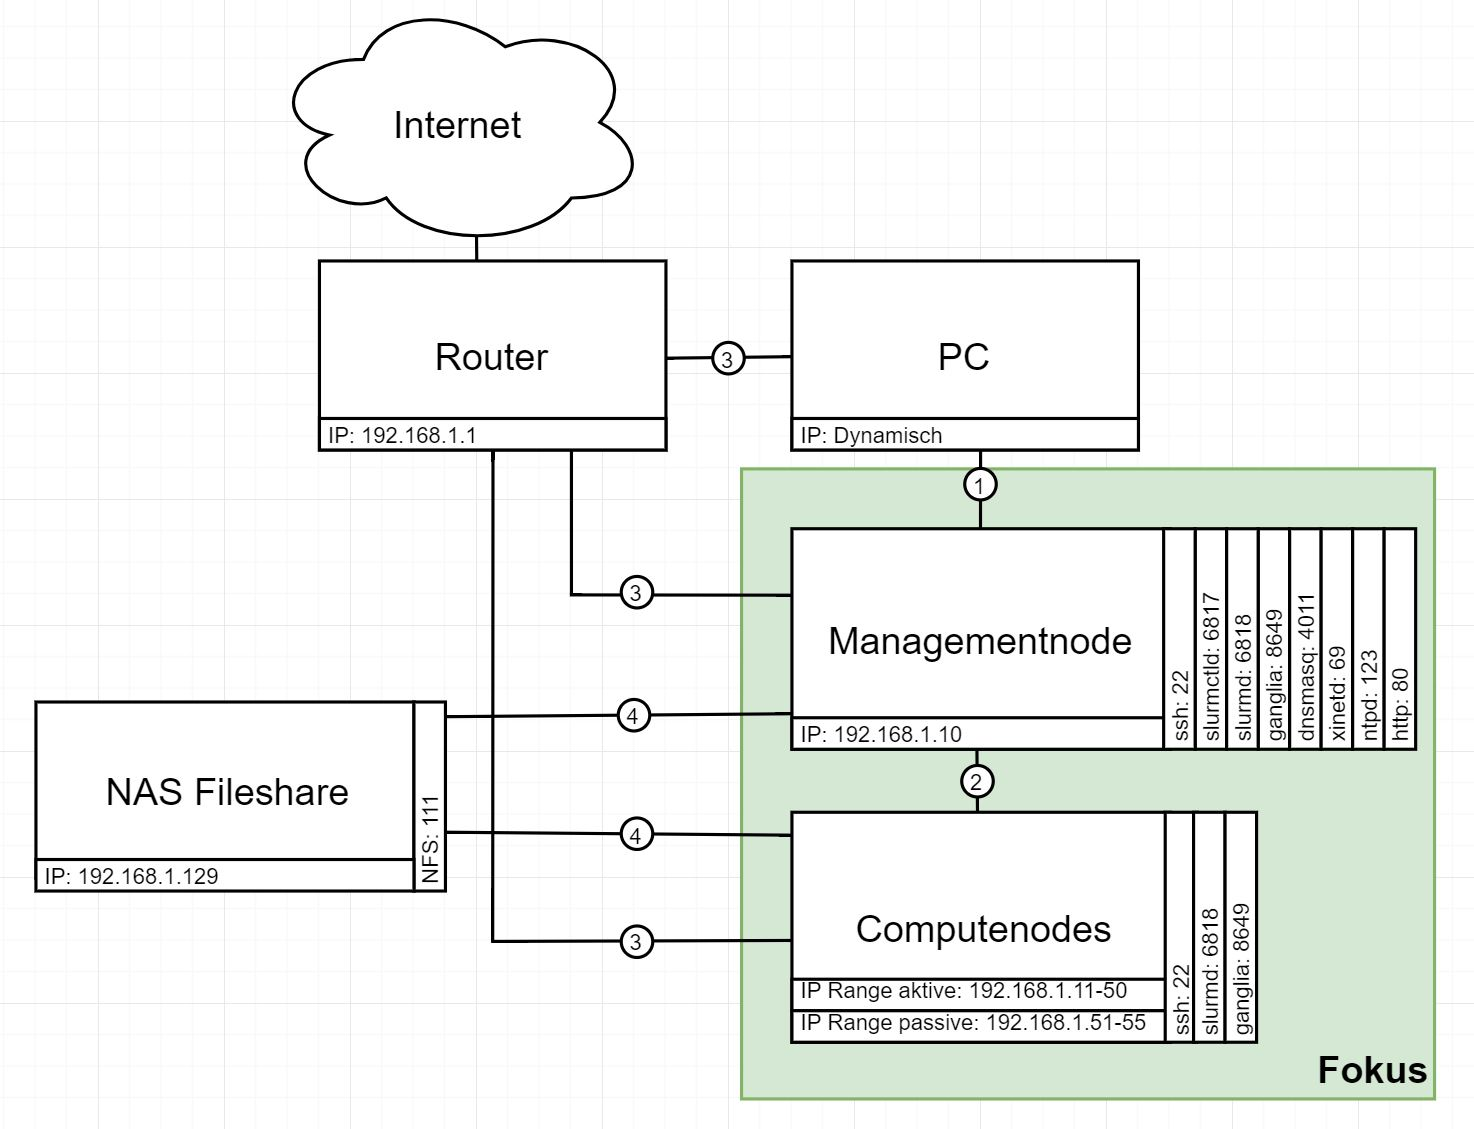
\includegraphics[scale=0.5]{tech_ueberblick.jpg}
\caption{Technischer Überblick}
\label{fig:Technischer Überblick}
\end{figure} 

\textbf{Beschreibung}\newline
Der grün markierte Teil beinhaltet das Vorhaben. Diese Komponenten werden neu in das Netzwerk eingebunden und aufgebaut. Die Komponenten ausserhalb des grünen Bereiches existieren bereits und es müssen für die Umsetzung konfigurationen vorgenommen werden.

\textbf{Verbindung 1} \newline
Der PC kann mit dem \textbf{SSH Protokoll} auf den Managementnode zugreifen. Dadurch kann die Installation vorgenommen werden. Zugleich wird über das \textbf{HTT Protokoll} via Webbrowser der Zugriff auf diverse Applikationen wie z.B. Nagios \& Ganglia ermöglicht.

\textbf{Verbindung 2} \newline
Der Managementnode verteilt via \textbf{dnsmasq} und dem \textbf {TFT Protkoll} das Betriebssystem an die Computenodes über das Netzwerk. Sogleich ist auch der \textbf{Slurm Controller} für die Jobsteuerung auf dem Managementnode installiert, welcher mit den \textbf{Slurm Daemons} auf den Computenodes kommuniziert. Weiterhin sind die Monitoring Komponenten \textbf{Ganglia und Nagios} auf dem Managementnode installiert, welche Daten von den Computenodes einfordern und zur Auswertung verarbeiten.

\textbf{Verbindung 3} \newline
Der Router verteilt via \textbf{DHCP} statische IP Adressen und Hostnamen welche per MAC Adressen gebunden sind.

\textbf{Verbindung 4} \newline
Der NAS Share wird mit dem \textbf{SMB} Protokoll auf den Compute und dem Masternode angehängt.

\subsubsection{Verwendete Protokolle}
\begin{table}[H]
\centering
\begin{tabular}{p{2cm}p{4cm}p{5cm}p{5cm}}
\hline
\rowcolor{heading} \textbf{Verbindung} & \textbf{Protokoll} & \textbf{Protokollfamilie} & \textbf{Ports} \\\hline
1 & SSH & TCP & 22 \\\hline
2 & SMTP & TCP & 25 \\\hline
3 & DHCP & UDP & 67 / 78 \\\hline
4 & TFTP & UDP & 69 \\\hline
5 & HTTP & TCP & 80 \\\hline
6 & SMB & TCP & 445 \\\hline
\end{tabular}
\caption{Protokolle}
\end{table}
